%%%%%%%%%%%%%%%%%%%%
%
% Combinatorics for the Lights Out 2x2 game
% 
% Authors: Valentin Montmirail and Marie Pelleau
%
%%%%%%%%%%%%%%%%%%%%

\documentclass{article}

\usepackage{fixmath}
\usepackage{pgf, tikz}

\usepackage[top = 0.75cm, bottom = 0cm, left = 2.5cm]{geometry}

\definecolor{bleu}{rgb}{0, 0.6, 0.8}
\definecolor{rose}{rgb}{0.8, 0, 0.4}

\title{Lights Out}

\author{}
\date{} 


\def\x{\mathbold{\textcolor{orange!80!red}{x}}}
\def\y{\mathbold{\textcolor{bleu}{y}}}
\def\z{\mathbold{\textcolor{green!70!blue}{z}}}
\def\t{\mathbold{\textcolor{rose}{t}}}

\begin{document}
  \Large
  \maketitle
  
  Lights Out is an electronic game released by Tiger Electronics in 1995.
  The game consists of a $5\times5$ grid of lights. 
  The game starts, a random number of lights are switched on. Pressing any of the lights will toggle it and its 4 adjacent lights.
  The goal of the game is to find the smallest combination of lights in order to switch all the lights off.
  
  \bigskip
  \textbf{Gameplay}
  
  \begin{center}
    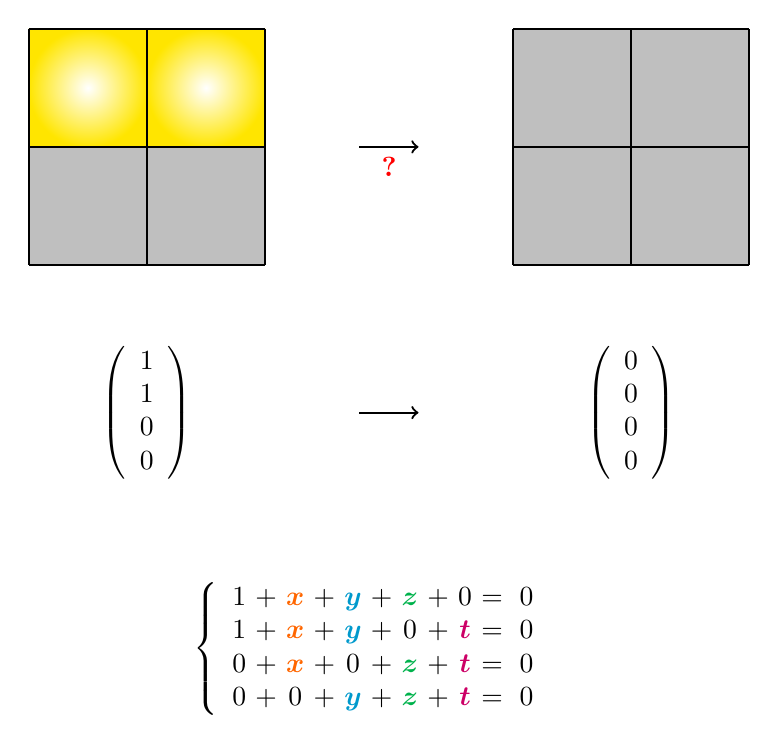
\begin{tikzpicture}[scale = 1.5]
      \fill[even odd rule, inner color = white, outer color = yellow!90!red] (0, 1) rectangle (1, 2);
      \fill[even odd rule, inner color = white, outer color = yellow!90!red] (1, 1) rectangle (2, 2);
      \fill[lightgray] (0, 0) rectangle (2, 1);
      \draw[step=1, thick] (0, 0) grid (2, 2);
      
      \draw[->, thick] (2.8, 1) -- (3.3, 1) node [midway, below] {\textcolor{red}{\textbf{?}}};
      
      \begin{scope}[xshift = 4.1cm]
        \fill[lightgray] (0, 0) rectangle (2, 2);
        \draw[step=1, thick] (0, 0) grid (2, 2);
      \end{scope}
      
      \draw (1, -1.25) node {$\left(\begin{array}{c}1\\1\\0\\0\end{array}\right)$};
      \draw[->, thick] (2.8, -1.25) -- (3.3, -1.25);
      \draw (5.1, -1.25) node {$\left(\begin{array}{c}0\\0\\0\\0\end{array}\right)$};
      
      \draw (2.85, -3.25) node {$\left\{\begin{array}{c @{~+~} c  @{~+~} c @{~+~} c @{~+~} c  @{~=~0}}
        1 & \x & \y & \z &  0\\
        1 & \x & \y &  0 & \t\\
        0 & \x &  0 & \z & \t\\
        0 &  0 & \y & \z & \t\end{array}\right.$};
    \end{tikzpicture}
  \end{center}
  
  \bigskip
  \textbf{Combinatorics}
  
  \begin{itemize}
    \item Best case: 0 light pressed (all the lights are already switched off).
    \item Worst case: for a $n \times n$ board, one must press on all the $n^2$ lights.
    \item Average case: $\displaystyle{\frac{n^2}{2} \times \frac{(2^{n^2)}}{(2^{n^2} - 1)}}$ (around half of the lights).
  \end{itemize}

\end{document}
